\documentclass[tikz,border=5pt]{standalone}
\usepackage{amsmath}
\usetikzlibrary{arrows.meta}

\begin{document}
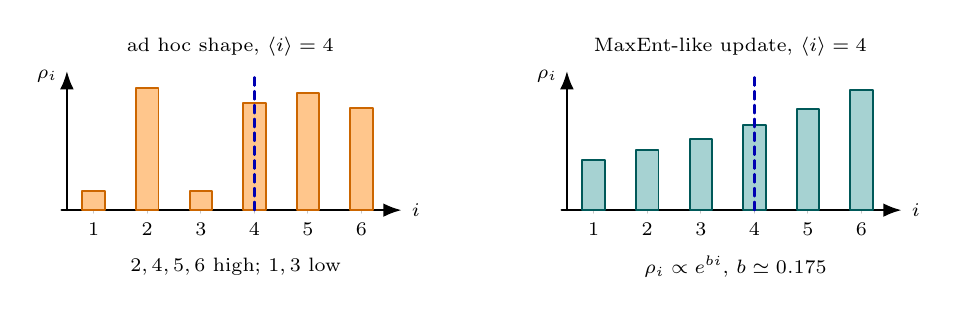
\begin{tikzpicture}[x=0.68cm,y=6.2cm,line cap=round,line join=round,>=Latex]

\def\barw{0.42}

\begin{scope}
    \node[font=\scriptsize] at (3.55,0.335) {ad hoc shape, $\langle i\rangle=4$};
    \draw[->,line width=0.8pt] (0.4,0) -- (6.75,0) node[right,font=\scriptsize] {$i$};
    \draw[->,line width=0.8pt] (0.5,0) -- (0.5,0.285);
    \node[font=\scriptsize,left] at (0.5,0.275) {$\rho_i$};
    \foreach \x in {1,...,6} {
        \draw[gray!45] (\x,0) -- (\x,-0.006);
        \node[font=\scriptsize,below] at (\x,-0.006) {$\x$};
    }
    \foreach \x/\h in {1/0.04,2/0.25,3/0.04,4/0.22,5/0.24,6/0.21} {
        \fill[orange!45] (\x-\barw/2,0) rectangle (\x+\barw/2,\h);
        \draw[orange!80!black,line width=0.7pt] (\x-\barw/2,0) rectangle (\x+\barw/2,\h);
    }
    \draw[densely dashed,blue!70!black,line width=0.85pt] (4,0) -- (4,0.275);
    \node[font=\scriptsize,align=center] at (3.65,-0.115) {$2,4,5,6$ high; $1,3$ low};
\end{scope}

\begin{scope}[xshift=6.35cm]
    \node[font=\scriptsize] at (3.55,0.335) {MaxEnt-like update, $\langle i\rangle=4$};
    \draw[->,line width=0.8pt] (0.4,0) -- (6.75,0) node[right,font=\scriptsize] {$i$};
    \draw[->,line width=0.8pt] (0.5,0) -- (0.5,0.285);
    \node[font=\scriptsize,left] at (0.5,0.275) {$\rho_i$};
    \foreach \x in {1,...,6} {
        \draw[gray!45] (\x,0) -- (\x,-0.006);
        \node[font=\scriptsize,below] at (\x,-0.006) {$\x$};
    }
    \foreach \x/\h in {1/0.103,2/0.123,3/0.146,4/0.174,5/0.207,6/0.247} {
        \fill[teal!35] (\x-\barw/2,0) rectangle (\x+\barw/2,\h);
        \draw[teal!70!black,line width=0.7pt] (\x-\barw/2,0) rectangle (\x+\barw/2,\h);
    }
    \draw[densely dashed,blue!70!black,line width=0.85pt] (4,0) -- (4,0.275);
    \node[font=\scriptsize,align=center] at (3.65,-0.115) {$\rho_i\propto e^{b i}$, $b\simeq0.175$};
\end{scope}

\end{tikzpicture}
\end{document}
